\documentclass{standalone}
\usepackage{tikz}
\usetikzlibrary{patterns, positioning}
\usepackage[sfdefault]{ClearSans} %% option 'sfdefault' activates Clear Sans as the default text font
\usepackage[T1]{fontenc}

\begin{document}
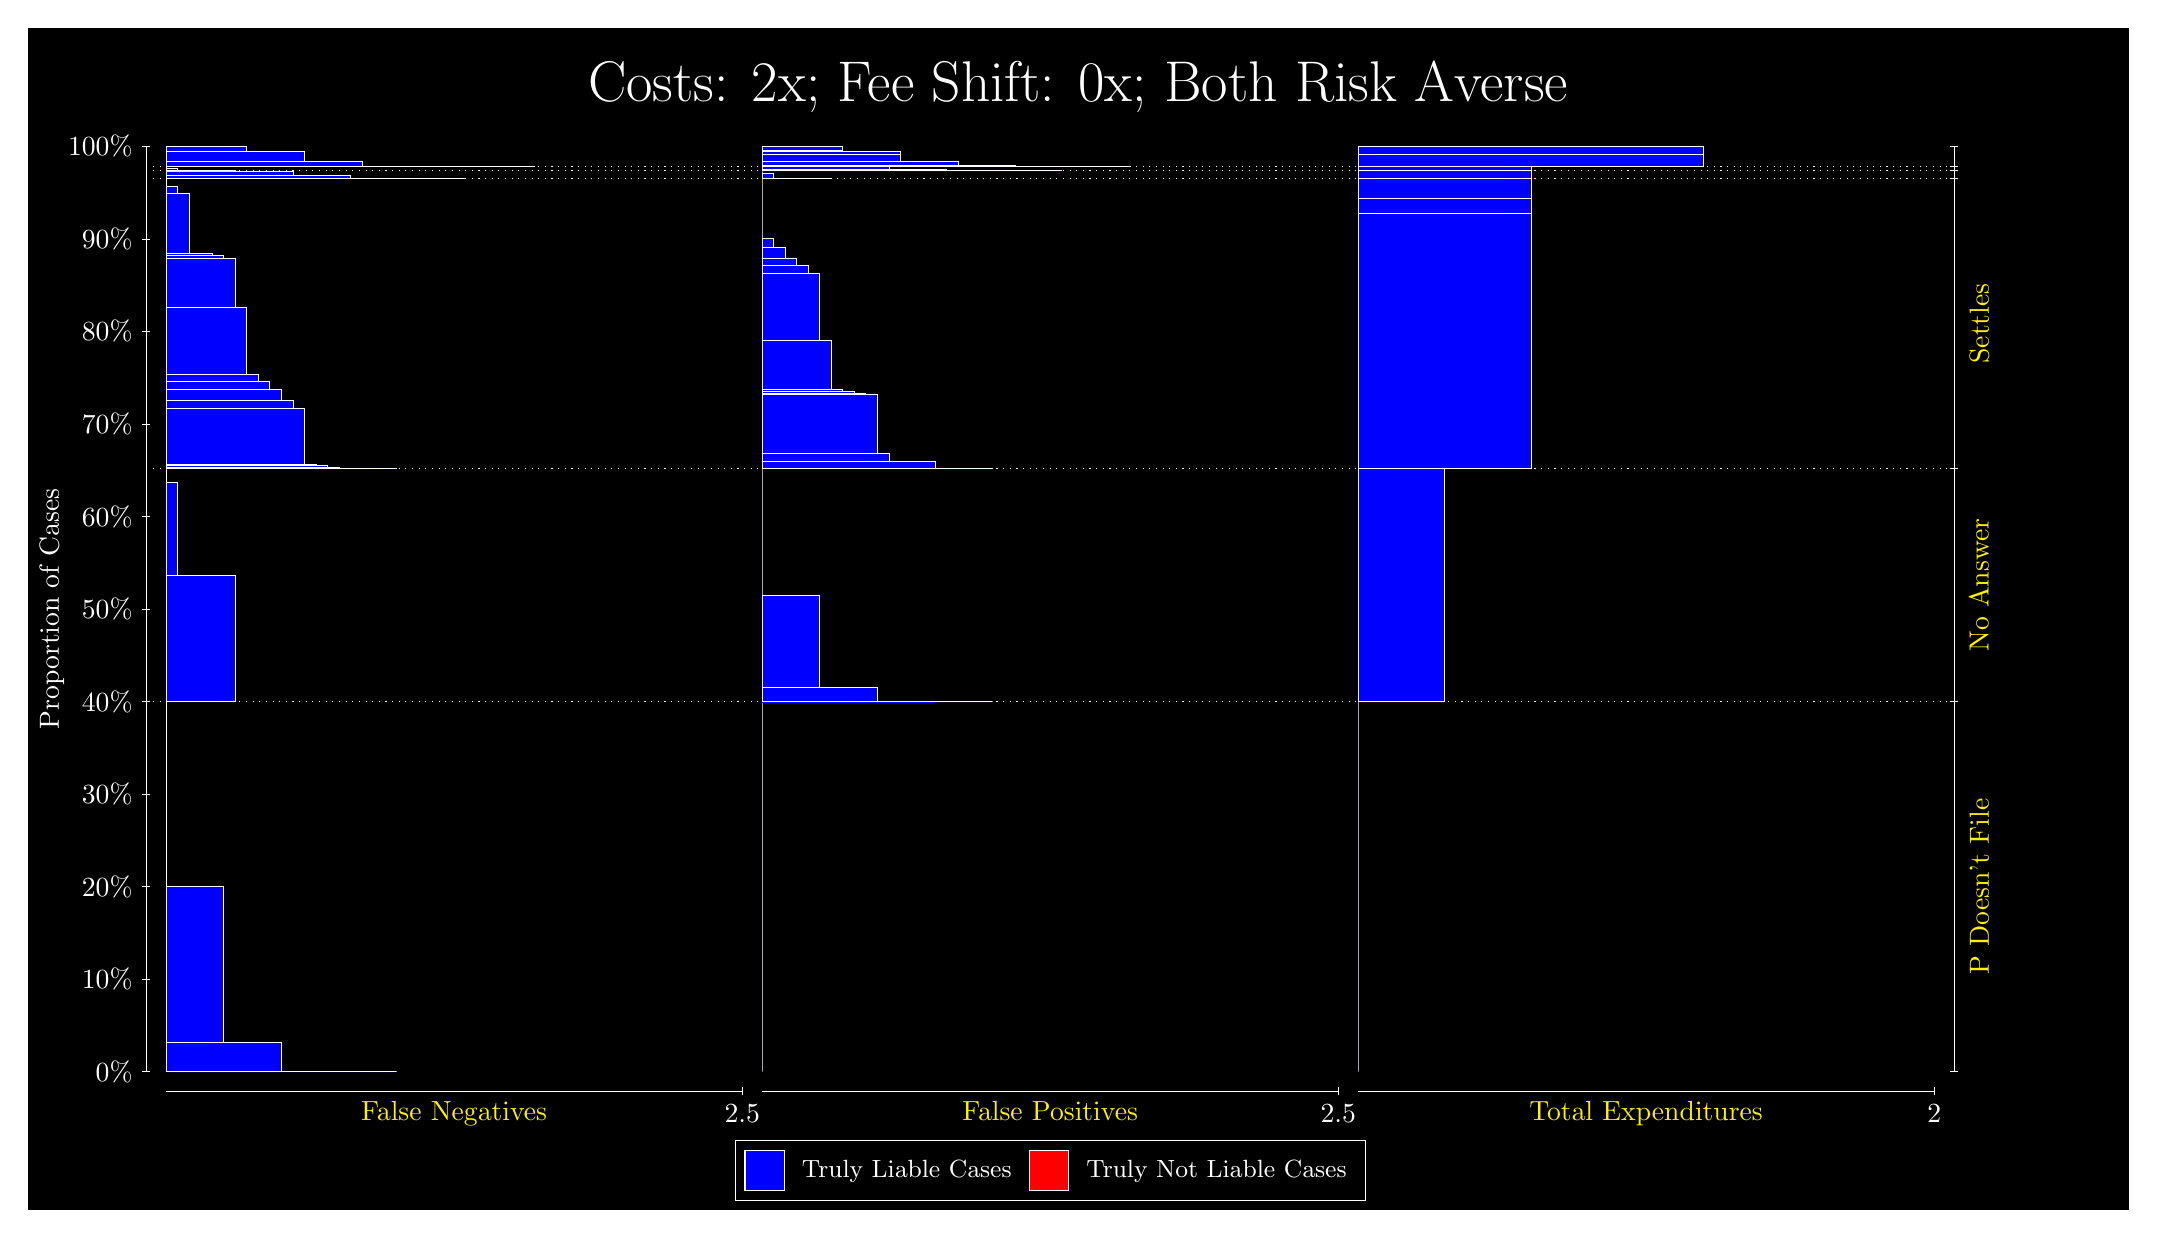
\begin{tikzpicture}
\draw[fill=black] (0,0) rectangle (26.667,15);
\draw[text=white] (0,13.5) rectangle (26.667,15) node[midway] {\huge Costs: 2x; Fee Shift: 0x; Both Risk Averse};
\draw[white, very thin] (1.5,1.75) -- (1.5,13.5);
\node[rotate=90, text=white, anchor=center] at (0.3, 7.625) {Proportion of Cases};
\draw[white, very thin] (1.45,1.75) -- (1.55,1.75);
\node[text=white, anchor=east] at (1.45, 1.75) {0\%};
\draw[white, very thin] (1.45,2.925) -- (1.55,2.925);
\node[text=white, anchor=east] at (1.45, 2.925) {10\%};
\draw[white, very thin] (1.45,4.1) -- (1.55,4.1);
\node[text=white, anchor=east] at (1.45, 4.1) {20\%};
\draw[white, very thin] (1.45,5.275) -- (1.55,5.275);
\node[text=white, anchor=east] at (1.45, 5.275) {30\%};
\draw[white, very thin] (1.45,6.45) -- (1.55,6.45);
\node[text=white, anchor=east] at (1.45, 6.45) {40\%};
\draw[white, very thin] (1.45,7.625) -- (1.55,7.625);
\node[text=white, anchor=east] at (1.45, 7.625) {50\%};
\draw[white, very thin] (1.45,8.8) -- (1.55,8.8);
\node[text=white, anchor=east] at (1.45, 8.8) {60\%};
\draw[white, very thin] (1.45,9.975) -- (1.55,9.975);
\node[text=white, anchor=east] at (1.45, 9.975) {70\%};
\draw[white, very thin] (1.45,11.15) -- (1.55,11.15);
\node[text=white, anchor=east] at (1.45, 11.15) {80\%};
\draw[white, very thin] (1.45,12.325) -- (1.55,12.325);
\node[text=white, anchor=east] at (1.45, 12.325) {90\%};
\draw[white, very thin] (1.45,13.5) -- (1.55,13.5);
\node[text=white, anchor=east] at (1.45, 13.5) {100\%};

\draw[white, very thin] (24.457,1.75) -- (24.457,13.5);
\draw[white, very thin] (24.407,1.75) -- (24.507,1.75);
\node[anchor=west] at (24.407, 1.75) {};
\draw[white, very thin] (24.407,6.4489) -- (24.507,6.4489);
\node[anchor=west] at (24.407, 6.4489) {};
\draw[white, very thin] (24.407,9.4082) -- (24.507,9.4082);
\node[anchor=west] at (24.407, 9.4082) {};
\draw[white, very thin] (24.407,13.092) -- (24.507,13.092);
\node[anchor=west] at (24.407, 13.092) {};
\draw[white, very thin] (24.407,13.191) -- (24.507,13.191);
\node[anchor=west] at (24.407, 13.191) {};
\draw[white, very thin] (24.407,13.248) -- (24.507,13.248);
\node[anchor=west] at (24.407, 13.248) {};
\draw[white, very thin] (24.407,13.5) -- (24.507,13.5);
\node[anchor=west] at (24.407, 13.5) {};

\draw[white, very thin, fill=blue] (1.75,1.75) rectangle (4.6775,1.75);
\draw[white, very thin, fill=blue] (1.75,1.75) rectangle (3.9457,1.7532);
\draw[white, very thin, fill=blue] (1.75,1.7532) rectangle (3.2138,2.126);
\draw[white, very thin, fill=blue] (1.75,2.126) rectangle (2.4819,4.1027);
\draw[white, very thin, fill=red] (1.75,4.1027) rectangle (1.75,4.1027);
\draw[white, very thin, fill=blue] (1.75,4.1027) rectangle (1.75,6.4489);
\draw[white, very thin, fill=blue] (1.75,6.4489) rectangle (2.6283,8.0564);
\draw[white, very thin, fill=blue] (1.75,8.0564) rectangle (1.8964,9.2296);
\draw[white, very thin, fill=red] (1.75,9.2296) rectangle (1.75,9.2296);
\draw[white, very thin, fill=blue] (1.75,9.2296) rectangle (1.75,9.4082);
\draw[white, very thin, fill=blue] (1.75,9.4082) rectangle (4.6775,9.4083);
\draw[white, very thin, fill=blue] (1.75,9.4083) rectangle (4.3848,9.4083);
\draw[white, very thin, fill=blue] (1.75,9.4083) rectangle (4.092,9.4085);
\draw[white, very thin, fill=blue] (1.75,9.4085) rectangle (3.9457,9.4274);
\draw[white, very thin, fill=blue] (1.75,9.4274) rectangle (3.7993,9.4517);
\draw[white, very thin, fill=blue] (1.75,9.4517) rectangle (3.6529,9.4566);
\draw[white, very thin, fill=blue] (1.75,9.4566) rectangle (3.5065,10.173);
\draw[white, very thin, fill=blue] (1.75,10.173) rectangle (3.3602,10.281);
\draw[white, very thin, fill=blue] (1.75,10.281) rectangle (3.2138,10.415);
\draw[white, very thin, fill=blue] (1.75,10.415) rectangle (3.0674,10.516);
\draw[white, very thin, fill=blue] (1.75,10.516) rectangle (2.921,10.607);
\draw[white, very thin, fill=blue] (1.75,10.607) rectangle (2.7746,11.462);
\draw[white, very thin, fill=blue] (1.75,11.462) rectangle (2.6283,12.081);
\draw[white, very thin, fill=blue] (1.75,12.081) rectangle (2.4819,12.114);
\draw[white, very thin, fill=blue] (1.75,12.114) rectangle (2.3355,12.139);
\draw[white, very thin, fill=blue] (1.75,12.139) rectangle (2.1891,12.143);
\draw[white, very thin, fill=blue] (1.75,12.143) rectangle (2.0428,12.902);
\draw[white, very thin, fill=blue] (1.75,12.902) rectangle (1.8964,12.996);
\draw[white, very thin, fill=red] (1.75,12.996) rectangle (1.75,12.996);
\draw[white, very thin, fill=blue] (1.75,12.996) rectangle (1.75,13.092);
\draw[white, very thin, fill=blue] (1.75,13.092) rectangle (5.5558,13.092);
\draw[white, very thin, fill=blue] (1.75,13.092) rectangle (4.8239,13.092);
\draw[white, very thin, fill=blue] (1.75,13.092) rectangle (4.092,13.129);
\draw[white, very thin, fill=blue] (1.75,13.129) rectangle (3.3602,13.189);
\draw[white, very thin, fill=blue] (1.75,13.189) rectangle (2.6283,13.191);
\draw[white, very thin, fill=red] (1.75,13.191) rectangle (1.75,13.191);
\draw[white, very thin, fill=blue] (1.75,13.191) rectangle (2.6283,13.191);
\draw[white, very thin, fill=blue] (1.75,13.191) rectangle (1.8964,13.227);
\draw[white, very thin, fill=red] (1.75,13.227) rectangle (1.75,13.227);
\draw[white, very thin, fill=blue] (1.75,13.227) rectangle (1.75,13.248);
\draw[white, very thin, fill=blue] (1.75,13.248) rectangle (6.4341,13.248);
\draw[white, very thin, fill=blue] (1.75,13.248) rectangle (5.7022,13.248);
\draw[white, very thin, fill=blue] (1.75,13.248) rectangle (4.9703,13.252);
\draw[white, very thin, fill=blue] (1.75,13.252) rectangle (4.2384,13.31);
\draw[white, very thin, fill=blue] (1.75,13.31) rectangle (3.5065,13.437);
\draw[white, very thin, fill=blue] (1.75,13.437) rectangle (2.7746,13.495);
\draw[white, very thin, fill=blue] (1.75,13.495) rectangle (2.0428,13.5);
\draw[white, very thin, fill=red] (1.75,13.5) rectangle (1.75,13.5);
\draw[white, very thin, fill=blue] (1.75,13.5) rectangle (1.75,13.5);
\draw[white, very thin, fill=red] (9.3189,1.75) rectangle (9.3189,1.75);
\draw[white, very thin, fill=blue] (9.3189,1.75) rectangle (9.3189,6.4489);
\draw[white, very thin, fill=red] (9.3189,6.4489) rectangle (12.246,6.4489);
\draw[white, very thin, fill=blue] (9.3189,6.4489) rectangle (12.246,6.4489);
\draw[white, very thin, fill=blue] (9.3189,6.4489) rectangle (11.515,6.4492);
\draw[white, very thin, fill=blue] (9.3189,6.4492) rectangle (10.783,6.6275);
\draw[white, very thin, fill=blue] (9.3189,6.6275) rectangle (10.051,7.8008);
\draw[white, very thin, fill=blue] (9.3189,7.8008) rectangle (9.3189,9.4082);
\draw[white, very thin, fill=red] (9.3189,9.4082) rectangle (12.246,9.4082);
\draw[white, very thin, fill=blue] (9.3189,9.4082) rectangle (12.246,9.4084);
\draw[white, very thin, fill=red] (9.3189,9.4084) rectangle (11.954,9.4084);
\draw[white, very thin, fill=blue] (9.3189,9.4084) rectangle (11.954,9.4084);
\draw[white, very thin, fill=red] (9.3189,9.4084) rectangle (11.661,9.4084);
\draw[white, very thin, fill=blue] (9.3189,9.4084) rectangle (11.661,9.4086);
\draw[white, very thin, fill=blue] (9.3189,9.4086) rectangle (11.515,9.5033);
\draw[white, very thin, fill=red] (9.3189,9.5033) rectangle (11.368,9.5033);
\draw[white, very thin, fill=blue] (9.3189,9.5033) rectangle (11.368,9.5033);
\draw[white, very thin, fill=blue] (9.3189,9.5033) rectangle (11.222,9.5033);
\draw[white, very thin, fill=red] (9.3189,9.5033) rectangle (11.075,9.5033);
\draw[white, very thin, fill=blue] (9.3189,9.5033) rectangle (11.075,9.5034);
\draw[white, very thin, fill=blue] (9.3189,9.5034) rectangle (10.929,9.5976);
\draw[white, very thin, fill=blue] (9.3189,9.5976) rectangle (10.783,10.356);
\draw[white, very thin, fill=blue] (9.3189,10.356) rectangle (10.636,10.361);
\draw[white, very thin, fill=blue] (9.3189,10.361) rectangle (10.49,10.386);
\draw[white, very thin, fill=blue] (9.3189,10.386) rectangle (10.344,10.418);
\draw[white, very thin, fill=blue] (9.3189,10.418) rectangle (10.197,11.037);
\draw[white, very thin, fill=blue] (9.3189,11.037) rectangle (10.051,11.893);
\draw[white, very thin, fill=blue] (9.3189,11.893) rectangle (9.9044,11.984);
\draw[white, very thin, fill=blue] (9.3189,11.984) rectangle (9.758,12.084);
\draw[white, very thin, fill=blue] (9.3189,12.084) rectangle (9.6116,12.219);
\draw[white, very thin, fill=blue] (9.3189,12.219) rectangle (9.4652,12.327);
\draw[white, very thin, fill=blue] (9.3189,12.327) rectangle (9.3189,13.092);
\draw[white, very thin, fill=red] (9.3189,13.092) rectangle (10.197,13.092);
\draw[white, very thin, fill=blue] (9.3189,13.092) rectangle (10.197,13.093);
\draw[white, very thin, fill=blue] (9.3189,13.093) rectangle (9.4652,13.154);
\draw[white, very thin, fill=blue] (9.3189,13.154) rectangle (9.3189,13.191);
\draw[white, very thin, fill=red] (9.3189,13.191) rectangle (13.125,13.191);
\draw[white, very thin, fill=blue] (9.3189,13.191) rectangle (13.125,13.191);
\draw[white, very thin, fill=blue] (9.3189,13.191) rectangle (12.393,13.191);
\draw[white, very thin, fill=blue] (9.3189,13.191) rectangle (11.661,13.212);
\draw[white, very thin, fill=blue] (9.3189,13.212) rectangle (10.929,13.247);
\draw[white, very thin, fill=blue] (9.3189,13.247) rectangle (10.197,13.248);
\draw[white, very thin, fill=red] (9.3189,13.248) rectangle (14.003,13.248);
\draw[white, very thin, fill=blue] (9.3189,13.248) rectangle (14.003,13.248);
\draw[white, very thin, fill=red] (9.3189,13.248) rectangle (13.271,13.248);
\draw[white, very thin, fill=blue] (9.3189,13.248) rectangle (13.271,13.248);
\draw[white, very thin, fill=red] (9.3189,13.248) rectangle (12.539,13.248);
\draw[white, very thin, fill=blue] (9.3189,13.248) rectangle (12.539,13.253);
\draw[white, very thin, fill=blue] (9.3189,13.253) rectangle (11.807,13.311);
\draw[white, very thin, fill=red] (9.3189,13.311) rectangle (11.807,13.311);
\draw[white, very thin, fill=blue] (9.3189,13.311) rectangle (11.807,13.311);
\draw[white, very thin, fill=blue] (9.3189,13.311) rectangle (11.075,13.393);
\draw[white, very thin, fill=red] (9.3189,13.393) rectangle (11.075,13.393);
\draw[white, very thin, fill=blue] (9.3189,13.393) rectangle (11.075,13.438);
\draw[white, very thin, fill=blue] (9.3189,13.438) rectangle (10.344,13.45);
\draw[white, very thin, fill=blue] (9.3189,13.45) rectangle (10.344,13.496);
\draw[white, very thin, fill=blue] (9.3189,13.496) rectangle (9.6116,13.496);
\draw[white, very thin, fill=blue] (9.3189,13.496) rectangle (9.6116,13.5);
\draw[white, very thin, fill=blue] (9.3189,13.5) rectangle (9.3189,13.5);
\draw[white, very thin, fill=red] (16.888,1.75) rectangle (16.888,1.75);
\draw[white, very thin, fill=blue] (16.888,1.75) rectangle (16.888,6.4489);
\draw[white, very thin, fill=red] (16.888,6.4489) rectangle (17.986,6.4489);
\draw[white, very thin, fill=blue] (16.888,6.4489) rectangle (17.986,9.4082);
\draw[white, very thin, fill=red] (16.888,9.4082) rectangle (19.083,9.4082);
\draw[white, very thin, fill=blue] (16.888,9.4082) rectangle (19.083,12.655);
\draw[white, very thin, fill=red] (16.888,12.655) rectangle (19.083,12.655);
\draw[white, very thin, fill=blue] (16.888,12.655) rectangle (19.083,12.842);
\draw[white, very thin, fill=red] (16.888,12.842) rectangle (19.083,12.842);
\draw[white, very thin, fill=blue] (16.888,12.842) rectangle (19.083,13.092);
\draw[white, very thin, fill=red] (16.888,13.092) rectangle (19.083,13.092);
\draw[white, very thin, fill=blue] (16.888,13.092) rectangle (19.083,13.191);
\draw[white, very thin, fill=red] (16.888,13.191) rectangle (19.083,13.191);
\draw[white, very thin, fill=blue] (16.888,13.191) rectangle (19.083,13.248);
\draw[white, very thin, fill=red] (16.888,13.248) rectangle (21.279,13.248);
\draw[white, very thin, fill=blue] (16.888,13.248) rectangle (21.279,13.405);
\draw[white, very thin, fill=red] (16.888,13.405) rectangle (21.279,13.405);
\draw[white, very thin, fill=blue] (16.888,13.405) rectangle (21.279,13.5);
\draw[white, dotted] (1.5,6.4489) -- (24.457,6.4489);
\draw[white, dotted] (1.5,9.4082) -- (24.457,9.4082);
\draw[white, dotted] (1.5,13.092) -- (24.457,13.092);
\draw[white, dotted] (1.5,13.191) -- (24.457,13.191);
\draw[white, dotted] (1.5,13.248) -- (24.457,13.248);
\draw[white, very thin] (1.75,1.5) -- (9.0689,1.5);
\node[text=yellow, anchor=north] at (5.4094, 1.5) {False Negatives};
\draw[white, very thin] (9.0689,1.45) -- (9.0689,1.55);
\node[text=white, anchor=north] at (9.0689, 1.45) {2.5};

\draw[white, very thin] (9.3189,1.5) -- (16.638,1.5);
\node[text=yellow, anchor=north] at (12.978, 1.5) {False Positives};
\draw[white, very thin] (16.638,1.45) -- (16.638,1.55);
\node[text=white, anchor=north] at (16.638, 1.45) {2.5};

\draw[white, very thin] (16.888,1.5) -- (24.207,1.5);
\node[text=yellow, anchor=north] at (20.547, 1.5) {Total Expenditures};
\draw[white, very thin] (24.207,1.45) -- (24.207,1.55);
\node[text=white, anchor=north] at (24.207, 1.45) {2};

\node[text=yellow, centered, rotate=90] at (24.777, 4.0995) {P Doesn't File};
\node[text=yellow, centered, rotate=90] at (24.777, 7.9286) {No Answer};
\node[text=yellow, centered, rotate=90] at (24.777, 11.25) {Settles};




\draw (12.978300999999998,1.5) node[draw=none] (baseCoordinate) {};
\begin{scope}[align=center]
        \matrix[scale=0.5, draw=white, below=0.5cm of baseCoordinate, nodes={draw}, column sep=0.1cm]{
            \node[rectangle, draw, minimum width=0.5cm, minimum height=0.5cm, fill=blue] {}; &
            \node[draw=none, font=\small, text=white] (B) {Truly Liable Cases}; &
            \node[rectangle, draw, minimum width=0.5cm, minimum height=0.5cm, fill=red] {}; &
            \node[draw=none, font=\small, text=white] (B) {Truly Not Liable Cases}; \\
            };
\end{scope}

\end{tikzpicture}
\end{document}